% TODO: Rename this header
\subsection{Main Logic}

To handle all logic

As mentioned in Section \ref{sec:parsing_tasks}, UpdateFromTestsRepo is run when someone pushes to \textit{tests}.
Since tasks and issues need to be synchronized every time this happens, all logic for doing so will happen there.

More specifically, we create the function handleTasks that manages all logic relating to tasks.
The function is supplied with every assignment created by UpdateFromTestsRepo
The function itself is run at the end of UpdateFromTestsRepo.

\lstinputlisting[caption={The function handleTasks, responsible for all task related logic}, 
                language=Golang, label={code:handleTasks}, firstline=64, lastline=95]{code/tasks.go}

The logic contained in this function will be explained in the following sections.

\begin{figure}[ht]
    \centering
    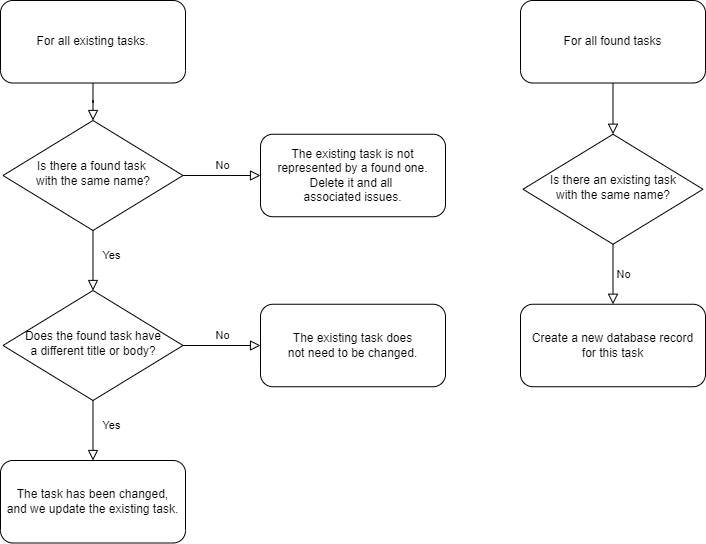
\includegraphics[width=\textwidth]{photos/synchronize-tasks-flow-chart.png}
    \caption{Flow chart describing how tasks are synchronized}
    \label{fig:synchronize-tasks-flow-chart}
\end{figure}